
% Springer LNCS template
\documentclass[runningheads]{llncs}

% ---------------- PACKAGES (LNCS-friendly) ----------------
\usepackage[T1]{fontenc}
\usepackage[utf8]{inputenc}

% Core + tables
\usepackage{graphicx}
\usepackage{booktabs}
\usepackage{tabularx}
\usepackage{array}
\usepackage{siunitx}
\usepackage{amsmath}
\usepackage{adjustbox}
\usepackage{multirow}
\usepackage{colortbl}


%\usepackage{natbib}


\usepackage{wrapfig}


% hyperlinks (load hyperref last)
\usepackage[hidelinks]{hyperref}



% ================== LNCS-safe micro spacing ==================
\usepackage{microtype}
\raggedbottom
\setlength{\abovecaptionskip}{3pt plus 1pt minus 1pt}
\setlength{\belowcaptionskip}{3pt plus 1pt minus 1pt}
\setlength{\textfloatsep}{8pt plus 2pt minus 2pt}
\setlength{\floatsep}{8pt plus 2pt minus 2pt}
\setlength{\intextsep}{8pt plus 2pt minus 2pt}


% ---------------- COLORS / MACROS ----------------
\definecolor{lightgray}{gray}{0.95}
\definecolor{midgray}{gray}{0.90}
\newcommand{\sig}[1]{\textbf{#1}} % bold significant values

% Consistent short references (LNCS uses "Fig.")
\newcommand{\figref}[1]{Fig.~\ref{#1}}
\newcommand{\tabref}[1]{Table~\ref{#1}}
\newcommand{\secref}[1]{Section~\ref{#1}}

% siunitx numeric alignment
\sisetup{
  detect-all,
  group-digits=false,
  table-number-alignment = center,
  round-mode = places,
  round-precision = 3,
  input-signs = +-,      % allow leading minus in S columns
  input-symbols = (),    % allow parentheses if needed
  table-align-text-post = false
}

% TabularX: ragged-right X column
\newcolumntype{Y}{>{\raggedright\arraybackslash}X}

% Conservative space tweaks LNCS typically tolerates
\setlength{\textfloatsep}{10pt plus 2pt minus 2pt}
\setlength{\floatsep}{10pt plus 2pt minus 2pt}
\setlength{\intextsep}{10pt plus 2pt minus 2pt}
\setlength{\abovecaptionskip}{3.5pt} % conservative
\setlength{\belowcaptionskip}{2pt}   % conservative

% ===== Submission toggle (appendices count towards 12 pages) =====
\newif\ifincludeappendix
\includeappendixfalse   % <- keep false for submission to meet 12-page limit

\begin{document}

%
\title{Exploring Cultural Variations in Moral Judgments with Large Language Models}
%
\titlerunning{Cultural Variations in Moral Judgments with LLMs}
% abbreviated title for running head
% DOUBLE-BLIND SUBMISSION - AUTHORS HIDDEN
%\author{Hadi Mohammadi\inst{1} \and
%Efthymia Papadopoulou\inst{1} \and
%Yasmeen F.S.S. Meijer\inst{1} \and
%Ayoub Bagheri\inst{1}}
\author{Anonymous Authors}
%
%\authorrunning{H. Mohammadi et al.}
\authorrunning{Anonymous}
% abbreviated author list for running head
%
%\institute{Department of Methodology and Statistics, Utrecht University, Utrecht, The Netherlands\\
%\email{\{h.mohammadi,a.bagheri\}@uu.nl}\\
%\email{evi.papado98@gmail.com, mijntje.meijer@live.nl}}

\institute{Anonymous Institution}
%
\maketitle              % typeset the header of the contribution
%
\begin{abstract}
Large Language Models (LLMs) have shown strong performance across many tasks, but their ability to capture culturally diverse moral values remains unclear. In this paper, we examine whether LLMs mirror variations in moral attitudes reported by the World Values Survey and the PEW Research Center's Global Attitudes Survey. We compare smaller monolingual and multilingual models (GPT-2, OPT, BLOOMZ, and Qwen) with recent instruction tuned models (GPT-4o, GPT-4o-mini, Gemma-2-9b-it, and Llama-3.3-70B-Instruct). Using log-probability-based~\emph{moral justifiability} scores, we correlate each model's outputs with survey data covering a broad set of ethical topics. Our results show that many earlier or smaller models often produce near-zero or negative correlations with human judgments. In contrast, advanced instruction tuned models (including GPT-4o and GPT-4o-mini) achieve substantially higher positive correlations, suggesting they better reflect real-world moral attitudes. While scaling model size and using instruction tuning improves alignment with cross-cultural moral norms, challenges remain for certain topics and regions. We discuss these findings in relation to bias analysis, training data diversity, and strategies for improving the cultural sensitivity of LLMs.

\keywords{Large Language Models (LLMs) \and Moral judgments \and Cultural variation \and Cross-Cultural Analysis \and Bias Detection}
\end{abstract}


\section{Introduction}
Over the past few years, LLMs have gained prominence in both academic and public discussions~\cite{Bender2021}. Advances in model performance have made LLMs appealing for diverse applications, such as social media content moderation, chatbots, content creation, real-time translation, search engines, recommendation systems, and automated decision-making. While modern LLMs (e.g., GPT-4) show strong performance, a critical concern is how these models may inherit biases, including gender, racial, or cultural biases, from their training data. LLMs can easily absorb such biases because they learn from large-scale text corpora containing entrenched stereotypes~\cite{Staczak2021,Karpouzis2024}.Recent work further examines whether LLMs capture cross-cultural moral judgments, reporting partial alignment alongside systematic blind spots across topics and regions~\cite{mohammadi2025morality}. Our study complements these findings by correlating model-derived justifiability scores with WVS and PEW across a broader mix of model families and elicitation settings.


These biases raise concerns about fairness, particularly in contexts requiring moral judgments. If an LLM is trained mostly on data that negatively or inaccurately portrays certain cultural groups, it may repeat that bias in its responses. As these models become more widespread and globally deployed, the risk of perpetuating cultural biases increases, especially when moral perspectives diverge from common norms or survey results. Recent research indicates that current LLMs often exhibit a Western-centric bias~\cite{adilazuarda2024towards}, underscoring the need to evaluate their cross-cultural validity.


It is crucial to determine whether LLMs accurately mirror the moral judgments observed across diverse cultures. Despite its importance, this issue has received limited attention~\cite{arora2023probing,liu2024multilingual}. Our study investigates whether both monolingual and multilingual Pre-trained Language Models (PLMs) can capture nuanced cultural norms. These norms include subtle ethical differences across regions, for example, the acceptance of alcohol consumption or differing attitudes on topics like abortion. Although recent research suggests that multilingual PLMs might capture broader cultural nuances, they often fall short of reflecting the moral subtleties present in less dominant cultural groups~\cite{Hammerl2022,papadopoulou2024}.

We examine this question using two well-known cross-cultural datasets: the World Values Survey (WVS)~\cite{Inglehart2014,Haerpfer2022}, and the PEW Research Center's Global Attitudes Survey, which includes a module on moral issues across many countries~\cite{Pew2023}. These surveys offer a detailed view of global moral and cultural norms, serving as a benchmark for comparing LLM outputs against human responses. By converting survey questions into prompts, we derive log-probability-based~\emph{moral justifiability} scores. We then compare these scores with survey-based consensus on various ethical issues (e.g., drinking alcohol, sex before marriage, abortion, homosexuality), allowing us to see how closely different model types and training approaches align with cultural norms. Evaluating how effectively LLMs represent cultural values has scholarly and practical significance. If a model systematically misrepresents certain moral perspectives, it may reinforce stereotypes or lead to biased outcomes. Conversely, culturally aware models can highlight shared values and nuanced disagreements, potentially contributing to more balanced dialogue. By comparing model outputs to reliable survey data, we identify areas where LLMs align with human values and highlight gaps in capturing diverse moral perspectives.

Our contributions are threefold: (1) We introduce a structured probing framework that leverages carefully designed prompts, contrasting moral statements, and log-probability-based scoring to assess how LLMs assign~\emph{justifiability} values to morally complex scenarios across cultures. (2) We empirically analyze the alignment between LLM-derived moral scores and human survey responses using correlation and clustering, highlighting where models reflect or deviate from real-world moral judgments. (3) We extend our evaluation to state-of-the-art instruction tuned and large-scale models, examining whether instruction tuning and scaling enhance alignment with cross-cultural moral norms. By identifying key strengths, weaknesses, and factors influencing model-human agreement, our work contributes to improved training data strategies, bias mitigation, and the development of culturally aware language models.


\section{Literature review}
%LLMs inherit biases present in their training data, and these biases can sometimes be amplified. Since LLMs are trained on extensive text corpora that reflect societal and cultural influences, they inevitably learn patterns that may reinforce existing disparities. This has raised concerns about fairness, representation, and the broader implications of deploying LLMs in real-world applications~\cite{Bender2021}.Moral judgments refer to evaluations of actions, intentions, or individuals as either acceptable or objectionable. These judgments vary widely by culture, shaped by religion, social norms, and historical factors~\cite{Haidt2001, Shweder1997}.


%\paragraph{Biases and Moral Judgments in LLMs.}
LLMs inherit biases embedded in their training data, and these biases can be amplified upon large-scale deployment. Because the underlying corpora often reflect entrenched social hierarchies, models run the risk of reproducing or even intensifying unfair patterns. Recent work has underscored this from multiple perspectives. For example, a 2025 study introduced a unified framework for transparency, fairness, and privacy in Artificial Intelligence (AI) pipelines~\cite{Radanliev2025}, while an interdisciplinary survey emphasized the importance of \emph{diversity, equity, and inclusion (DEI)} as prerequisites for trustworthy AI~\cite{cachat2023diversity}. Taken together with earlier warnings about opaque language-model behaviors~\cite{Bender2021}, these findings illustrate the need for technical innovation alongside social safeguards. In addition to high-level ethical governance, explainability-oriented methods can support bias analysis and mitigation at the text level~\cite{mohammadi2025explainability}. For instance, explanation-guided token replacement has been shown to steer LLM outputs away from problematic attributions while preserving utility~\cite{mohammadi2025xtr}. Beyond dataset and architectural factors, the reliability of LLM-produced judgments and annotations is itself uneven across demographic slices~\cite{mohammadi2025reliability}, reinforcing the need for careful evaluation protocols alongside fairness safeguards.


Moral judgments, evaluations of actions, intentions, or individuals as acceptable or objectionable, differ widely by culture, shaped by religious traditions, social norms, and historical contexts~\cite{Haidt2001,Shweder1997}. Understanding how pluralistic values are embedded in contemporary LLMs remains a pressing research concern.  As noted by~\cite{Graham2016}, Western, Educated, Industrialized, Rich, and Democratic (W.E.I.R.D.) societies emphasize individual rights and autonomy, while non-W.E.I.R.D. societies often stress communal responsibilities and spiritual considerations. Consequently, people in W.E.I.R.D. cultures may view personal choices like sexual behavior as an individual right, while those in non-W.E.I.R.D. cultures consider them a collective moral concern. Although many moral values overlap across cultures, there are also areas of genuine divergence, often referred to as \emph{moral value pluralism}~\cite{Johnson2022,Benkler2023}. However,~\cite{Kharchenko2024} argue that LLMs struggle to capture pluralistic moral values because their training data lacks sufficient cultural variety. Likewise,~\cite{Du2024} point out that the heavy use of English data in LLMs training limits the representation and creativity of models in other languages, although larger training corpora and bigger model architectures can improve performance.~\cite{arora2023probing} suggest that multilingual LLMs could learn cultural values by incorporating multilingual data in their training. Yet, the limited diversity within multilingual corpora can still cause these models to perform inconsistently across languages and cultural contexts.~\cite{Benkler2023} emphasize that many current AI systems lean toward the dominant values of Western cultures, especially English-speaking ones, leading to an implicit assumption that W.E.I.R.D. values are universal.

During training, LLMs use word embeddings to learn semantic and syntactic relationships based on how frequently words co-occur. These embeddings can encode the same social biases found in the training data~\cite{nemani2024gender,mohammadi2025explainability}. This association-based learning can produce biased outputs that influence the model's fairness and reliability. For instance, ~\cite{Johnson2022} showed that GPT-3 used the term \emph{Muslims} in violent contexts more often than \emph{Christians}, reinforcing damaging stereotypes. In all these cases, biased outputs can influence public perceptions and decisions, highlighting the importance of bias detection and mitigation~\cite{Noble2018,Zou2018}.
%

Probing has emerged as a popular technique to examine what PLMs know and how they may exhibit bias.~\cite{Ousidhoum2021} used probing to detect hateful or toxic content toward specific communities, while~\cite{nadeem2021stereoset} used context-based association tests to investigate stereotypes.~\cite{arora2023probing} adapted cross-cultural survey questions into prompts to test multilingual PLMs in 13 languages, discovering that these models often failed to match the moral values embedded in their training languages. Although there are multiple probing approaches, from \emph{cloze-style} tasks to \emph{pseudo-log-likelihood} scoring~\cite{nadeem2021stereoset,Salazar2019}, each has limitations. A simpler method directly computes the probability of specific tokens, following the original transformer design~\cite{Vaswani2017}.


Research on AI ethics underscores the need for models that respect cultural distinctions and support equitable treatment~\cite{Zowghi2023,cachat2023diversity,Karpouzis2024,Meijer2024}. Yet, biases in training data or architectural choices can lead to inconsistent handling of inputs from various backgrounds, raising doubts about an AI system's fairness and applicability~\cite{Karpouzis2024}. While studies like~\cite{arora2023probing} and \cite{Benkler2023} find that LLMs often struggle to accurately reflect diverse moral perspectives, others such as~\cite{ramezani2023knowledge} indicate that LLMs can sometimes capture considerable cultural variety. Similarly,~\cite{cao2023assessing} showed that ChatGPT aligns strongly with American cultural norms while adapting less effectively to others, reinforcing concerns of Western-centric bias in LLM outputs. This discrepancy highlights the need for more research on how LLMs learn and represent moral values in different cultural settings. Even though LLMs can inherit some cultural biases, the extent of their cross-cultural fidelity remains an open question~\cite{caliskan2017semantics}, with recent work suggesting partial improvements through balanced multilingual data, cultural prompting, and tailored evaluation frameworks, but also revealing persistent Western-centric tendencies across regions~\cite{alkhamissi-etal-2024-investigating,naous-etal-2024-beer,li2024culturellm,tao2024cultural,liu2025value,kwok2024adaptability,sachdeva2025normative}.




\section{Materials and methods}
\subsection{Data}
\label{sec:data}

To evaluate cross-cultural moral attitudes, we use two datasets: WVS Wave~7 and the PEW Research Center Global Attitudes Survey 2013. Each dataset's moral questions are labeled with topic codes. 
%See Table~\ref{tab:topic_mapping} in Appendix~\ref{appendix:topic_codes} for a full reference.

The WVS conducted from 2017 to 2020\footnote{\url{https://www.worldvaluessurvey.org/WVSDocumentationWV7.jsp}}, which covers respondents from 55 countries~\cite{Inglehart2014,Haerpfer2022}. We use the section of the survey dealing with Ethical Values and Norms. In this section, participants were asked to rate the \emph{justifiability} of 19 different behaviors or issues with moral connotations. These include topics such as \emph{divorce}, \emph{euthanasia}, \emph{political violence}, \emph{cheating on taxes}, and others. We performed preprocessing by filtering the dataset to retain only the responses to the 19 moral questions (Q177 to Q195) and the country code for each respondent.


Each response is an integer from 1 to 10. We then mapped the country codes to country names (using the provided codebook) so that each respondent entry includes their country and their answers to the moral questions. Next, we handled missing or non-response values. Entries coded as \(-1\), \(-2\), \(-4\), or \(-5\)~(i.e., \emph{Don't know}, \emph{No answer}, \emph{Not asked}, and \emph{Missing}) were set to \(0\), so they would not distort later calculations. We then grouped the data by country and averaged the responses for each moral statement. This yields a country-level average moral approval score for each of the 19 issues. Because different countries may use the \(1\)–\(10\) scale differently (culturally, some may avoid extreme ratings, etc.), and to facilitate comparison with the second dataset, we normalized these country mean scores to a range of \([-1, 1]\), with \(-1\) denoting \emph{never justifiable} and \(+1\) denoting \emph{always justifiable}.

After these steps, the WVS data provides, for each country and each moral topic, a score between -1 and 1 representing how acceptable that behavior is on average according to that country's respondents. Higher scores mean the society tends to view the behavior as more acceptable or justifiable, whereas lower scores mean it is seen as less acceptable or not justifiable. We treat these normalized \emph{country-by-topic} scores as the empirical ground truth of moral attitudes.

% \begin{figure}[t]
%   \centering
%   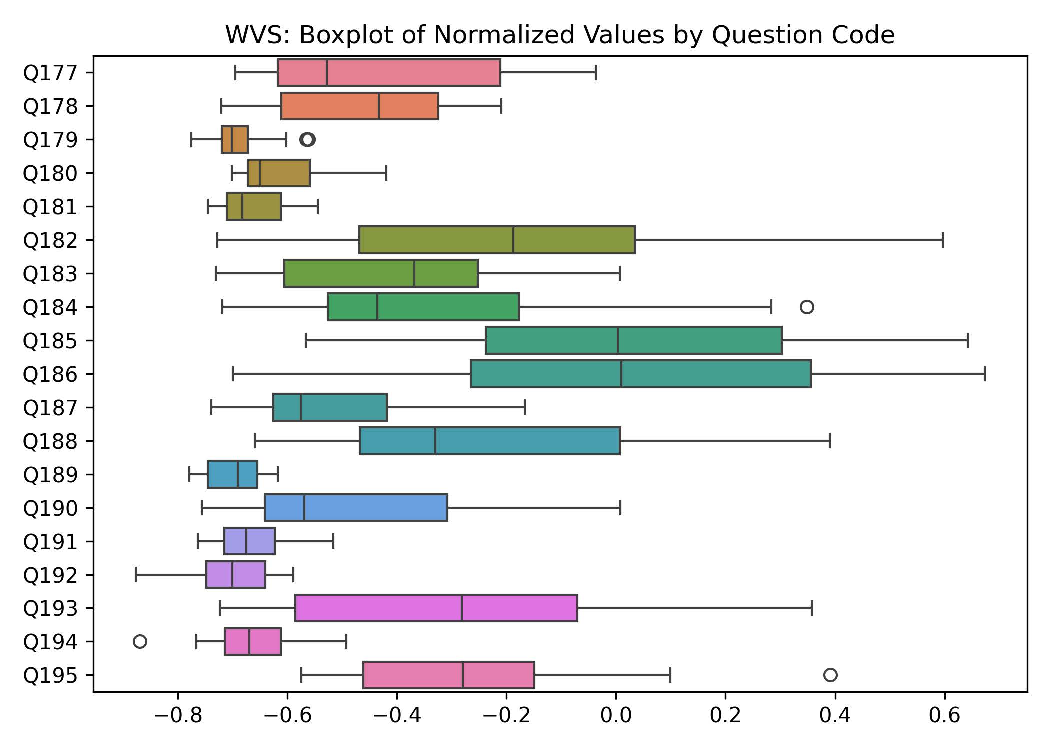
\includegraphics[width=0.66\textwidth]{figures/WVS_boxplot.pdf}
%   \caption{Spread of country mean scores across moral topics in the WVS Wave 7 dataset.}
%   \label{fig:wvs_figures_2}
% \end{figure}



%Figure~\ref{fig:wvs_figures_2} shows the spread of responses across different moral topics and countries. In other words, for each moral topic, how varied are the country scores? Some topics might have very similar scores in every culture (indicating global agreement), while others show a wide range (indicating high cross-cultural controversy).


\paragraph{PEW Global Attitudes Survey 2013} The PEW collected responses on moral issues from 39 countries, with about 100 respondents per country for the relevant questions\footnote{\url{https://www.pewresearch.org/dataset/spring-2013-survey-data/}}. Unlike WVS, which used a 10-point scale, the PEW survey questions were simpler: for each issue, respondents were asked whether the behavior is \emph{morally acceptable}, \emph{morally unacceptable}, or \emph{not a moral issue}.

From the PEW dataset, we extracted the questions corresponding to those eight moral topics (Q84A to Q84H). We again retained only the country identifier and these responses for our purposes. We coded the responses in a numeric way to be analogous to the WVS scale: for each question, we assigned a value of \(+1\) to \emph{morally acceptable}, \(-1\) to \emph{morally unacceptable}, and \(0\) to \emph{not a moral issue} and all non-responses (including \emph{Depends on situation}, \emph{Refused}, and \emph{Don't know}). As with WVS, we grouped responses by country, averaged them for each topic, and normalized the averages to \([-1, 1]\). %Figure~\ref{fig:pew_figures_2} shows the normalized PEW values across the eight moral questions. The comparison of normalized scores for WVS and PEW by country is also presented in Appendix~\ref{appendix:WVS_PEW_scores_by_country}, Figure~\ref{fig:dist_by_country}.


% \begin{figure}[t]
%   \centering
%   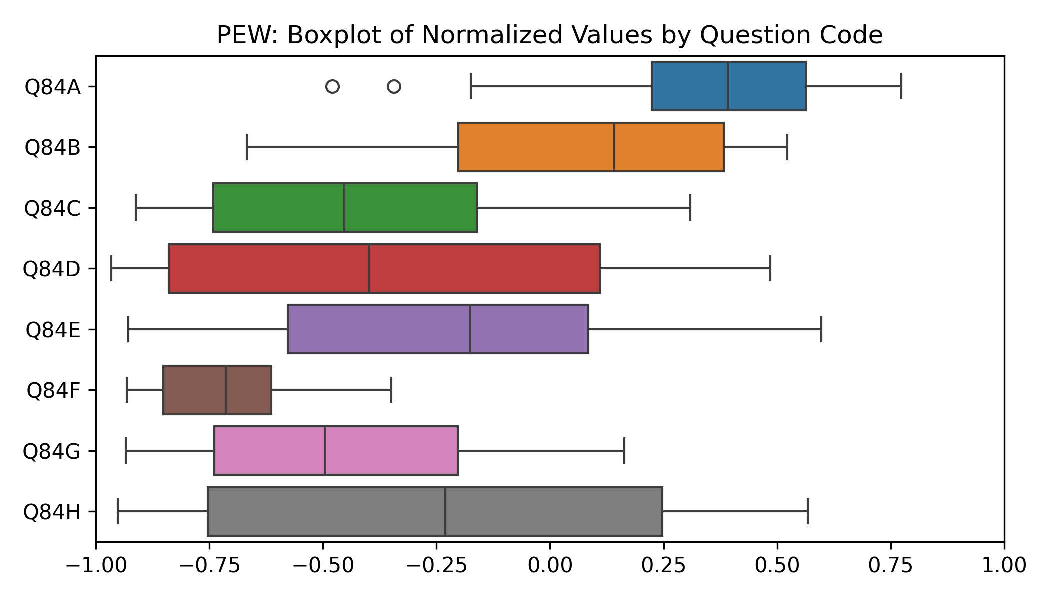
\includegraphics[width=0.70\textwidth]{figures/PEW_boxplot.pdf}
%   \caption{Spread of country mean scores across moral topics in the PEW 2013 dataset.}
%   \label{fig:pew_figures_2}
% \end{figure}


\subsection{Methodology}

Our evaluation of LLMs involves generating moral judgment scores from the models and comparing them with the two survey data. We first outline the LLMs we selected for testing, then describe how we prompted the models to obtain moral scores for each country and topic. Finally, we detail the three evaluation methods (\emph{correlation analysis}, \emph{cluster alignment analysis}, and \emph{models' error analysis}) that we applied to quantify the models' performance.

%\footnote{We will release our code upon acceptance to facilitate reproducibility.}

\paragraph{Model Selection}
We evaluated a broad range of transformer-based, decoder-only language models for their capacity to reflect cross-cultural moral judgments in the WVS and PEW data. Our initial set included the GPT-2 family (\texttt{GPT2-B}, \texttt{GPT2-M}, \texttt{GPT2-L})~\cite{Radford2019} for its coherent text generation at modest scales, as well as \texttt{OPT-125} and \texttt{OPT-350}~\cite{Zhang2022} to examine mid-sized behavior on ethically sensitive content. For multilingual coverage, we tested \texttt{BloomZ}~\cite{Muennighoff2023}, \texttt{Qwen-0.5B}, and \texttt{Qwen-72B}~\cite{Bai2023}, aiming to see whether broader linguistic training influences moral alignment. We then studied whether larger parameter sizes or instruction tuning could improve consistency by including \texttt{Gemma-2-9B-IT}~\cite{Mesnard2024}, \texttt{Llama-3-8B}, \texttt{Llama-3.3-70B-Instruct}~\cite{Touvron2023a}, and \texttt{Llama-2-70B}~\cite{Touvron2023b}. Additional instruction tuned models, such as \texttt{DBRX-Inst}~\cite{Conover2023a}, \texttt{MPT-30B}~\cite{MosaicML2023}, \texttt{Falcon3-7B}, \texttt{Falcon-40B-Inst}~\cite{Almazrouei2023}, \texttt{GPT-NeoX-20B}~\cite{Black2022}, \texttt{T5-Large}~\cite{raffel2020exploring}, and \texttt{Dolly-v2-12B}~\cite{Conover2023b}, covered diverse training setups and parameter scales. We further compared \texttt{Bloom} \cite{LeScao2022} and \texttt{BloomZ}~\cite{Muennighoff2023} to see how instruction-specific methods affect moral responses. Finally, we examined chat-focused or proprietary systems like \texttt{GPT‑3.5}~\cite{brown2020language}, \texttt{GPT‑4o}~\cite{OpenAI2024b}, and \texttt{GPT‑4o‑mini}~\cite{OpenAI2024a} to determine how interactive or closed-source models handle moral content. Importantly, none of these models received additional fine-tuning on moral or cultural data, meaning our findings show their unmodified views on ethical prompts.

\paragraph{Prompt Structuring}
Following the template-based probing framework introduced by~\cite{ramezani2023knowledge} for fine-grained moral-norm inference across cultures, we adapt and extend their basic method to probe a wider range of LLMs.
To query the models about moral judgments, we designed prompts that mimic the structure of statements about morality in different countries. Our goal was to get the model to complete statements in a way that reveals whether it thinks a behaviour is viewed as moral or immoral in a given culture. We used two main prompt templates for each country–topic pair:

% \\
% {\small {P1: \emph{In \(\{country\}\), \(\{topic\}\) is \(\{judgment\}\).}}},\\
% {\small {P2: \emph{People in \(\{country\}\) believe \(\{topic\}\) is \(\{judgment\}\).}}}
% \\

%\vspace{0.5em} % Optional: adds vertical space
{\small \textit{P1: In \(\{country\}\), \(\{topic\}\) is \(\{judgment\}\).}}\\
{\small \textit{P2: People in \(\{country\}\) believe \(\{topic\}\) is \(\{judgment\}\).}}

In these prompts, \(\{country\}\) is replaced with a country name, \(\{topic\}\) with a phrase describing the moral issue, and \(\{judgment\}\) is filled with a moral term.


 \paragraph{Moral Judgment Scores} We compute a moral score from the model for each country-topic. Let \(\mathcal{L}\) be a language model. For each moral topic (e.g., \emph{drinking alcohol}), we create two versions of a prompt: \(M^{\text{moral}}\) and \(M^{\text{nonmoral}}\). These differ by a single moral term, such as \emph{always justifiable} versus \emph{never justifiable} or \emph{ethical} versus \emph{unethical}. We then obtain $ log p\bigl(M^{\text{moral}}\bigr)\quad\text{and}\quad logp\bigl(M^{\text{nonmoral}}\bigr),$ which represent \(\mathcal{L}\)'s tendency toward each stance. To reduce the impact of specific word choices, we repeat this process with five moral-adjective pairs \footnote{Always justifiable vs. never justifiable, right vs. wrong, morally good vs. morally bad, ethically right vs. ethically wrong, and ethical vs. unethical} and compute the average difference in log probabilities:
$
\Delta \;=\; \log p\bigl(M^\text{moral}\bigr) \;-\; \log p\bigl(M^\text{nonmoral}\bigr).
$
\vspace{4pt}
\\
We apply min--max normalization to \(\Delta\) across all topics and countries, mapping \(\Delta\) into \([-1, +1]\):
$\Delta_{\text{norm}} \;=\; 2\,\frac{\Delta - \Delta_{\min}}{\Delta_{\max} - \Delta_{\min}} \;-\; 1.
$
\vspace{4pt}
\\
The result is a model-based \emph{moral justifiability score} \(s_i \in [-1, +1]\). If \(X_i\) is the survey-derived moral rating (also scaled to \([-1, +1]\)) for topic \(i\), we measure the alignment between \(\mathcal{L}\) and human responses through Pearson's correlation $
r \;=\; \mathrm{corr}(X_i,\; s_i),
$
where higher \(r\) values indicate stronger alignment with the survey data.

\paragraph{Direct Numerical Rating}
In contrast, for proprietary chat models (e.g., \texttt{GPT4o} and \texttt{GPT4o-mini}), the OpenAI ChatCompletion API does not provide access to token-level log probabilities. Instead, we adopt a direct elicitation approach. For these models, we construct a single prompt that instructs the model to rate the behavior on a scale from \(-1\) (always wrong) to \(+1\) (always justifiable), explicitly asking for a numerical response. Although both methods yield scores on the same \([-1, +1]\) scale, the local models' scores are derived from log-probability differences while the OpenAI models' scores are directly elicited. Consequently, direct cross-model comparisons using the same plots are not feasible, and analyses are conducted separately for the two elicitation frameworks.

\paragraph{Cross-Country Correlations and Clustering}
We compare each model's cross-country correlations on a given topic to the survey-based scores. This correlation analysis shows whether a model senses that certain issues polarize particular cultures. In addition, we represent each country as a vector of moral justifiability scores and apply clustering metrics (e.g., Adjusted Rand Index or Adjusted Mutual Information) to see if a model's country clusters match survey-derived groupings.


\paragraph{Comparative Prompts}
We explicitly ask the model to compare two countries' moral judgments on a given topic. We use a direct comparative prompt of the form: {{\emph{Regarding the morality of \(\{topic\}\), \(\{country X\}\) and \(\{country Y\}\) are similar.}}} This tests whether the model recognizes that some pairs of countries hold similar moral views on certain topics. Overall, our pipeline of constructing moral descriptors, calculating log-probability differences, and normalizing them gives a quantitative measure of how well each language model agrees with cross-cultural moral data.

\section{Results}

\subsection{Correlation Analysis}

\paragraph{Pearson correlations}
We quantify alignment with survey responses using Pearson’s $r$ on WVS and PEW. \tabref{tab:AllCorrelationsStars} summarizes results across families and scales. Proprietary and instruction tuned models (e.g., \texttt{GPT‑4o/‑mini}, \texttt{Gemma‑2‑9B‑IT}, \texttt{Falcon‑40B‑Inst}) show the strongest positive correlations on both datasets, whereas several earlier or base models (e.g., \texttt{Qwen‑0.5B}, \texttt{Llama‑2‑70B}) tend to score near zero or negative, indicating weaker reflection of survey‑measured norms.

% -------------------- Table 1 (wrapped, compact, LNCS-friendly) --------------------
\begin{wraptable}{r}{0.60\textwidth}
  \vspace{-0.8em}
  \centering
  \scriptsize
  \caption{\textbf{Correlation with survey scores.} Pearson $r$ between model predictions and WVS/PEW. Higher is better; stars denote significance.}
  \label{tab:AllCorrelationsStars}
  \setlength{\tabcolsep}{4pt}
  \begin{tabular}{@{} l r S[table-format=+1.3] l S[table-format=+1.3] l @{}}
    \toprule
    \textbf{Model} & \textbf{Params} &
      \multicolumn{2}{c}{\textbf{WVS}} &
      \multicolumn{2}{c}{\textbf{PEW}} \\
    \cmidrule(lr){3-4}\cmidrule(lr){5-6}
     & & {$r$} & \textit{Sig.} & {$r$} & \textit{Sig.} \\
    \midrule
    % --- GPT-2 family
    GPT2-B             & 117M &  0.210  & *** &  0.163  & **  \\
    GPT2-M             & 355M &  0.161  & *** & -0.094  &     \\
    GPT2-L             & 774M &  0.007  &     & -0.256  & *** \\
    \midrule
    % --- OPT
    OPT-125            & 125M &  0.016  &     &  0.127  & *   \\
    OPT-350            & 350M & -0.156  & *** & -0.334  & *** \\
    \midrule
    % --- Multilingual
    BloomZ             & 560M & \multicolumn{1}{c}{--} &     & \bfseries 0.443  & *** \\
    BLOOM              & 176B & -0.048  &     & \multicolumn{1}{c}{--} &     \\
    Qwen-0.5B          & 500M & -0.408  & *** &  0.029  &     \\
    Qwen-72B           & 72B  & -0.078  & *   & -0.060  &     \\
    \midrule
    % --- Llama
    Llama-2-70B        & 70B  & -0.329  & *** & -0.602  & *** \\
    Llama-3-8B         & 8B   &  0.161  & *** &  0.151  & **  \\
    Llama-3.3-70B-Inst & 70B  &  0.036  &     & -0.038  &     \\
    \midrule
    % --- Instruction tuned (open)
    Gemma-2-9B-IT      & 9B   & \bfseries 0.440 & *** & \bfseries 0.573 & *** \\
    Falcon3-7B         & 7B   & -0.312  & *** & -0.415  & *** \\
    Falcon-40B-Inst    & 40B  &  0.385  & *** & \bfseries 0.671 & *** \\
    GPT-NeoX-20B       & 20B  & -0.078  & *   &  0.001  &     \\
    Dolly-v2-12B       & 12B  & -0.247  & *** &  0.010  &     \\
    \midrule
    % --- Proprietary
    GPT-3.5            & --   & \bfseries 0.543 & *** & \bfseries 0.566 & *** \\
    GPT-4o             & --   & \bfseries 0.504 & *** & \bfseries 0.618 & *** \\
    GPT-4o-mini        & --   & \bfseries 0.472 & *** & \bfseries 0.678 & *** \\
    \bottomrule
  \end{tabular}
  \vspace{0.25\baselineskip}
  \parbox{0.60\textwidth}{\footnotesize\emph{Notes.} * $p{<}.05$, ** $p{<}.01$, *** $p{<}.001$.
  Bold indicates $r \ge 0.4$. “--” = not available.}
  \vspace{-0.6em}
\end{wraptable}
% ---------------------------------------------------------------------------

\paragraph{Country‑level correlations}
For each country $i$, with model vector $\mathbf{m}_i$ (topics) and survey vector $\mathbf{s}_i$, we compute $r_i=\mathrm{corr}(\mathbf{m}_i,\mathbf{s}_i)$. Summarizing across countries: on \texttt{WVS}, instruction tuned mid scale models are predominantly positive across many countries, whereas some large \texttt{Llama} variants frequently yield near‑zero or negative $r_i$. On \texttt{PEW}, no single model dominates all regions e.g., \texttt{Falcon‑40B‑Inst} is relatively strong in several MENA countries, while other regions show mixed alignment.

%(e.g., \texttt{Gemma‑2‑9B‑IT})

\paragraph{Pairwise model similarity}
We correlate log‑probability difference vectors across all (country, topic) pairs to obtain a model‑by‑model similarity matrix. Families cluster as expected (e.g., \texttt{GPT2‑B/M/L} together), while instruction tuned or very large models often diverge, reflecting distinct stance patterns; see \figref{fig:pairwise}.

\begin{figure}[ht]
  \centering
  \begin{minipage}[t]{0.49\textwidth}
    \centering
    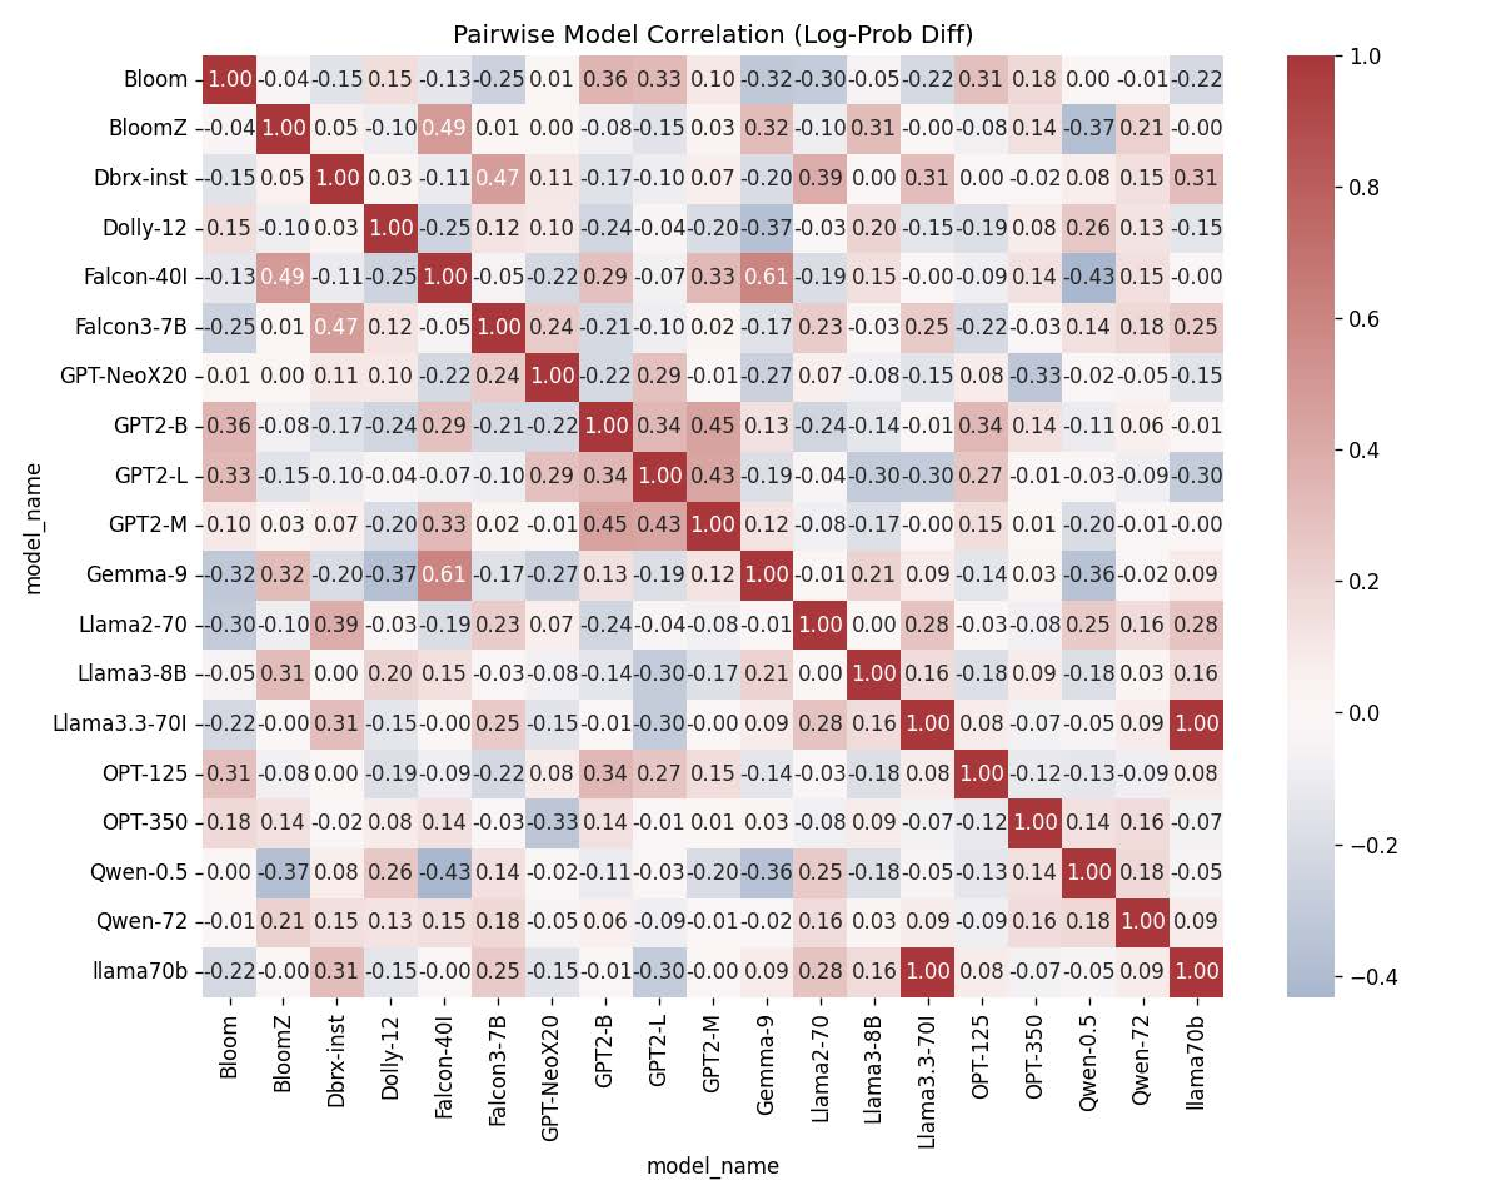
\includegraphics[width=\linewidth]{figures/model_pairwise_correlation_WVS.pdf}
  \end{minipage}\hfill
  \begin{minipage}[t]{0.49\textwidth}
    \centering
    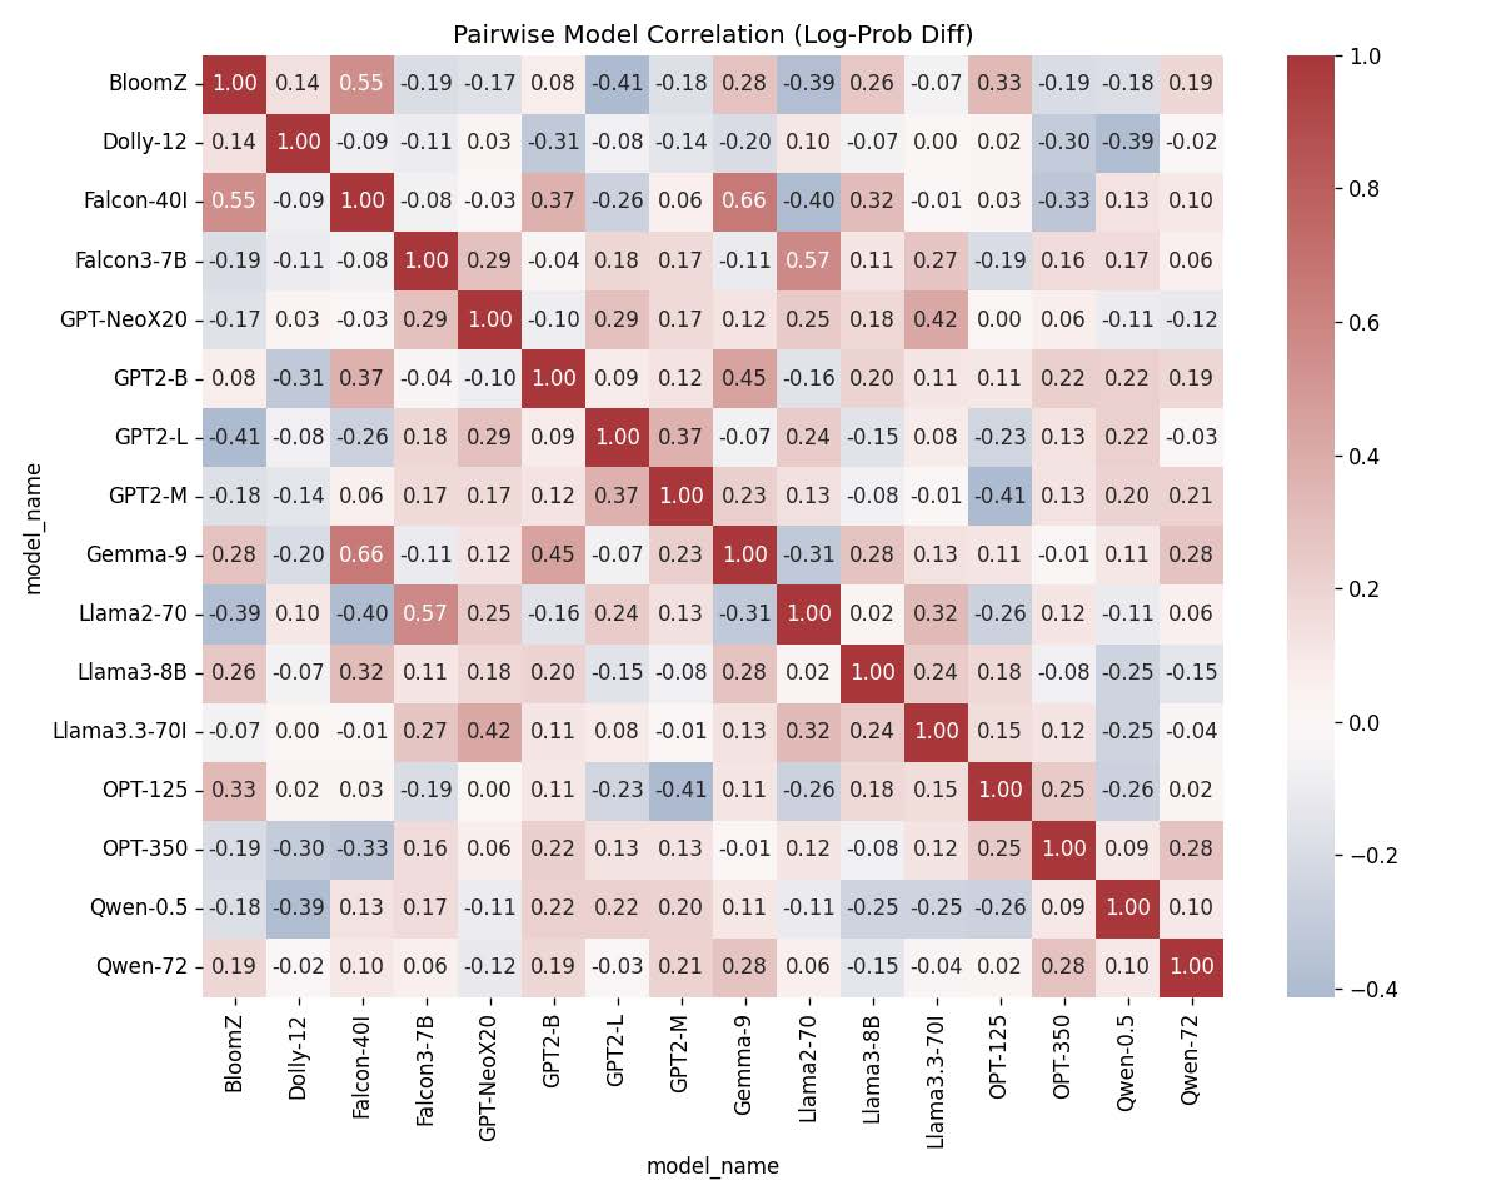
\includegraphics[width=\linewidth]{figures/model_pairwise_correlation_PEW.pdf}
  \end{minipage}
  \caption{\textbf{Pairwise similarity across models.} Correlations of log‑probability differences for WVS (left) and PEW (right). Warmer colors denote stronger agreement.}
  \label{fig:pairwise}
\end{figure}


\subsection{Cluster Alignment}
We created hierarchical clustering trees using the pairwise correlations (distance $d(X,Y)=1-\rho_{X,Y}$). The dendrograms in \figref{fig:hier} show that families cluster as expected (e.g., \texttt{GPT2-*} together), while instruction tuned or very large models (e.g., \texttt{GPT‑4o}) often merge only at higher linkages, reflecting distinct moral stance patterns across datasets. On WVS (left), \texttt{GPT2‑L/M/B} cluster at low linkage heights, with \texttt{Bloom}/\texttt{OPT‑125M}/\texttt{Llama‑3‑8B} forming a nearby group. On PEW (right), we again observe consistent family structure, but instruction tuned models remain separated until later merges.

In Figure~\ref{fig:hier} (left), models like \texttt{GPT2-Large} and \texttt{GPT2} are closely grouped, with \texttt{GPT2-Medium} merging slightly higher. A second cluster includes \texttt{Bloom}, \texttt{OPT-125}, and \texttt{Llama3-8B}, showing some shared correlation. Meanwhile, \texttt{Qwen-0.5}, \texttt{Qwen-72}, and \texttt{dolly-v2-12b} form another moderate distance group, while large-scale or instruction tuned models (e.g., \texttt{GPT3.5-turbo}, \texttt{GPT4o}, \texttt{Falcon-40I}) merge only at the top, suggesting limited similarity in their log-probability difference vectors. Figure~\ref{fig:hier} (right) shows a similar structure, with some clusters differing based on the models' responses to the morally focused PEW prompts. Notably, \texttt{GPT2} and \texttt{Gemma-9} cluster at low linkage heights, indicating strong similarities in their probability assignments for morally charged statements. Another cluster includes \texttt{Llama2-70}, \texttt{Falcon3-7B}, and \texttt{GPT-NeoX20}, which may reflect shared training data or architectural features leading to comparable moral stances.

\begin{figure}[t]
  \centering
  \begin{minipage}[t]{0.49\textwidth}
    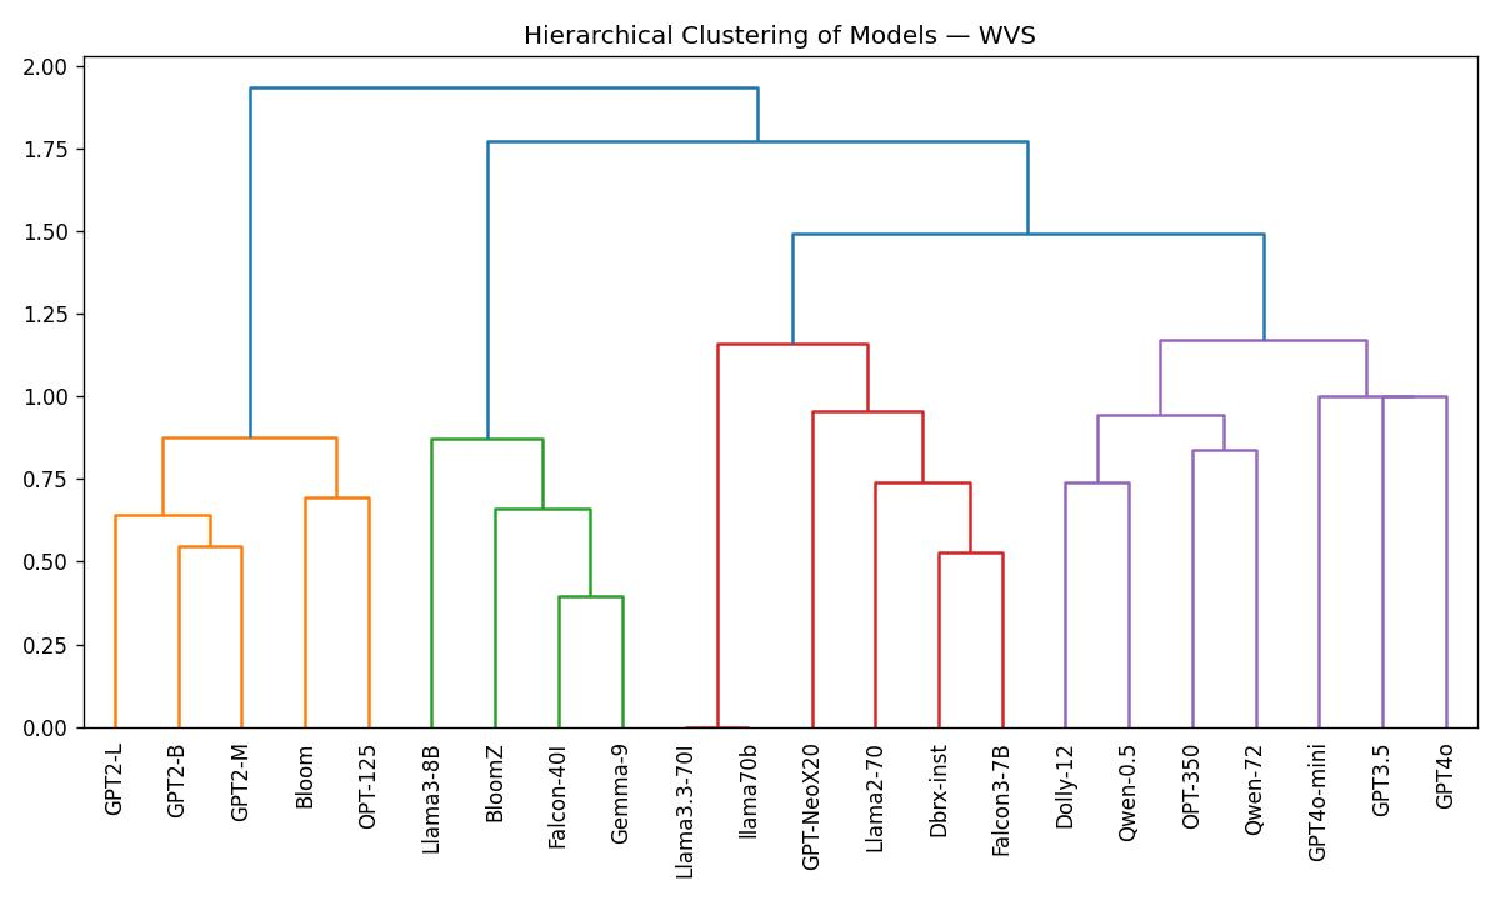
\includegraphics[width=\linewidth]{figures/hier_dendrogram_WVS.pdf}
  \end{minipage}\hfill
  \begin{minipage}[t]{0.49\textwidth}
    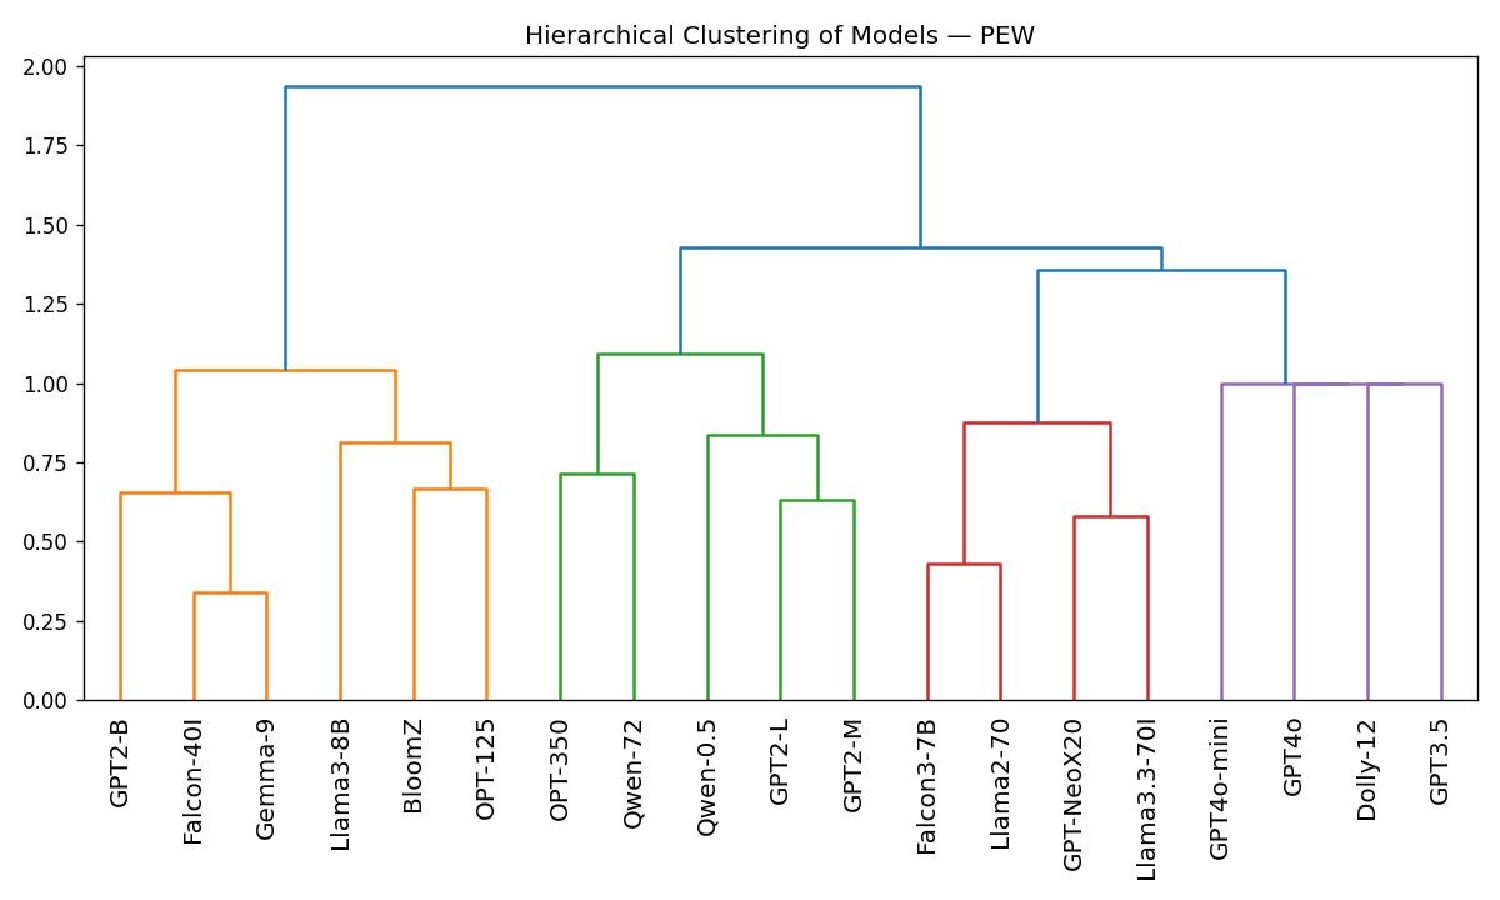
\includegraphics[width=\linewidth]{figures/hier_dendrogram_PEW.pdf}
  \end{minipage}
  \caption{Hierarchical clustering dendrograms based on model‑wise distances for WVS (left) and PEW (right).}
  \label{fig:hier}
\end{figure}

\vspace{-0.8em}
\subsection{Model Error Analysis}


\paragraph{Absolute Error}
To assess each model's deviation from human survey responses, we calculated $|\text{survey\_score}-\text{model\_prediction}|$ for each country–topic pair. \figref{fig:abs_error_dist} summarizes the distributions. Across WVS (left) in \figref{fig:abs_error_dist}, many predictions fall within 0.2–0.6, with a tail beyond 1.0 on culturally sensitive topics. PEW (right) shows a similar pattern, with most errors in 0.2–1.0 and a smaller mass above 1.5–2.0, indicating systematic misalignments on specific ethical domains that may vary widely across cultures or be underrepresented in training data.

%For WVS (left), many predictions fall within 0.2–0.6, with a tail beyond 1.0 on culturally sensitive topics. PEW (right) shows a similar pattern, with most errors in 0.2–1.0 and a smaller mass above 1.5–2.0.


\begin{figure}[t]
  \centering
  \begin{minipage}[t]{0.49\textwidth}
    \centering
    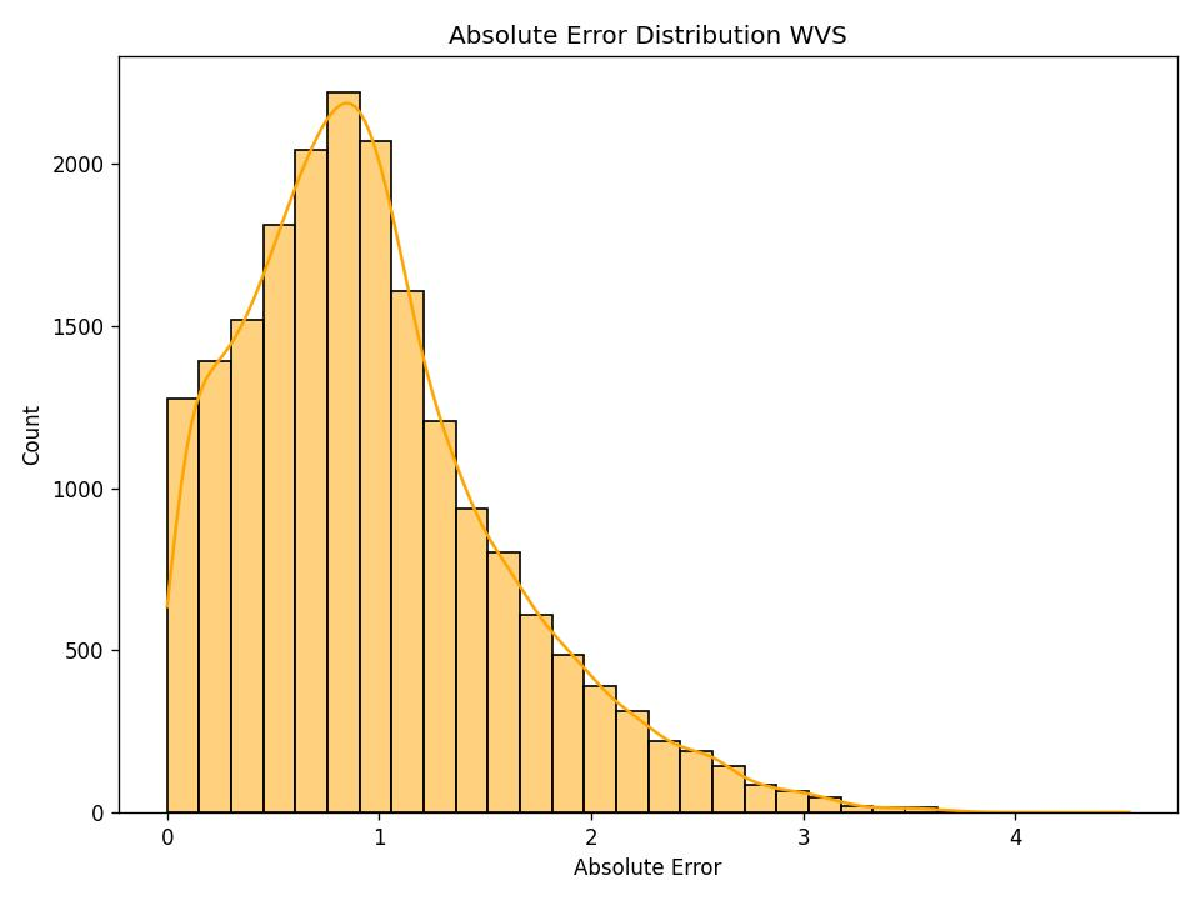
\includegraphics[width=\linewidth]{figures/abs_error_dist_WVS.pdf}
  \end{minipage}\hfill
  \begin{minipage}[t]{0.49\textwidth}
    \centering
    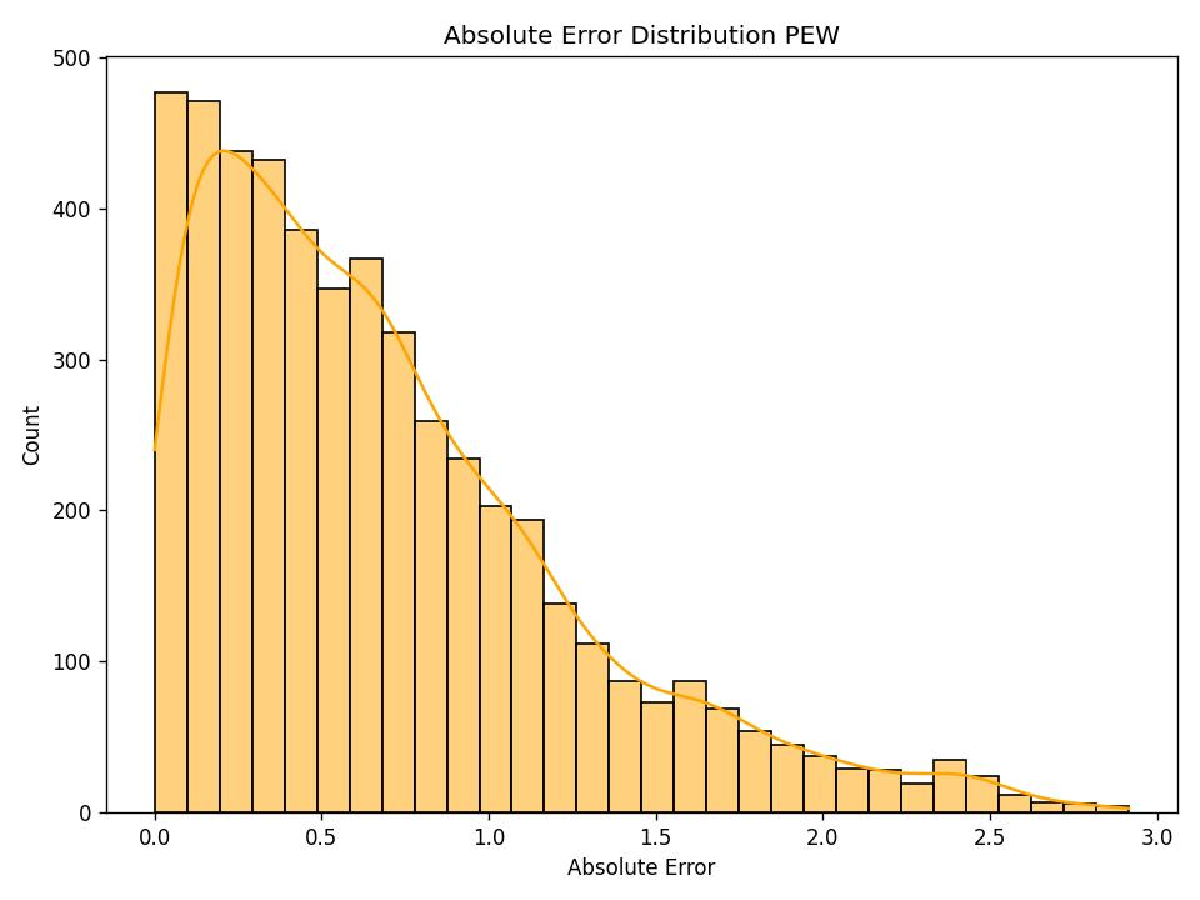
\includegraphics[width=\linewidth]{figures/abs_error_dist_PEW.pdf}
  \end{minipage}
  \caption{\textbf{Absolute‑error distributions.} $|\text{survey} - \text{model}|$ aggregated across models for WVS (left) and PEW (right).}
  \label{fig:abs_error_dist}
\end{figure}





\paragraph{Mean Absolute Error} While correlation captures how well each model's normalized outputs align with survey responses, we also examine the Mean Absolute Error (MAE) per (\textit{model}, \textit{topic}) pair. This highlights which moral topics each model finds "harder" (higher error) or "easier" (lower error). Figure~\ref{fig:heatmap} displays a heatmap across models (columns) and topics (rows) with darker cells indicating higher error, and Tables~\ref{tab:EasiestTopics} and \ref{tab:HardestTopics} show the ten easiest and hardest topics, respectively, based on average error.

In Figure~\ref{fig:heatmap}, topics like \emph{political violence}, \emph{suicide}, and \emph{stealing property} result in high errors for multiple models, whereas issues such as \emph{drinking alcohol}, \emph{using contraceptives}, and \emph{divorce} are generally easier for systems to manage. In Table~\ref{tab:EasiestTopics}, lists the ten topics with the lowest mean absolute error; within this group, the largest error is 0.51 for \emph{using contraceptives} and the smallest is 0.36 for \emph{death penalty}. Even the largest error among these ‘easy’ topics is still much lower than the errors observed for the more challenging topics in~\ref{tab:HardestTopics}. A low standard deviation indicates that most models agree on the ease of a topic, while a high standard deviation suggests that only some models find it easy. In contrast, Table~\ref{tab:HardestTopics} highlights that \emph{political violence} leads the list with an average error of 0.95. This is followed by \emph{suicide}, \emph{stealing property}, and \emph{accepting a bribe while on duty}.

\begin{figure}[t]
  \centering
  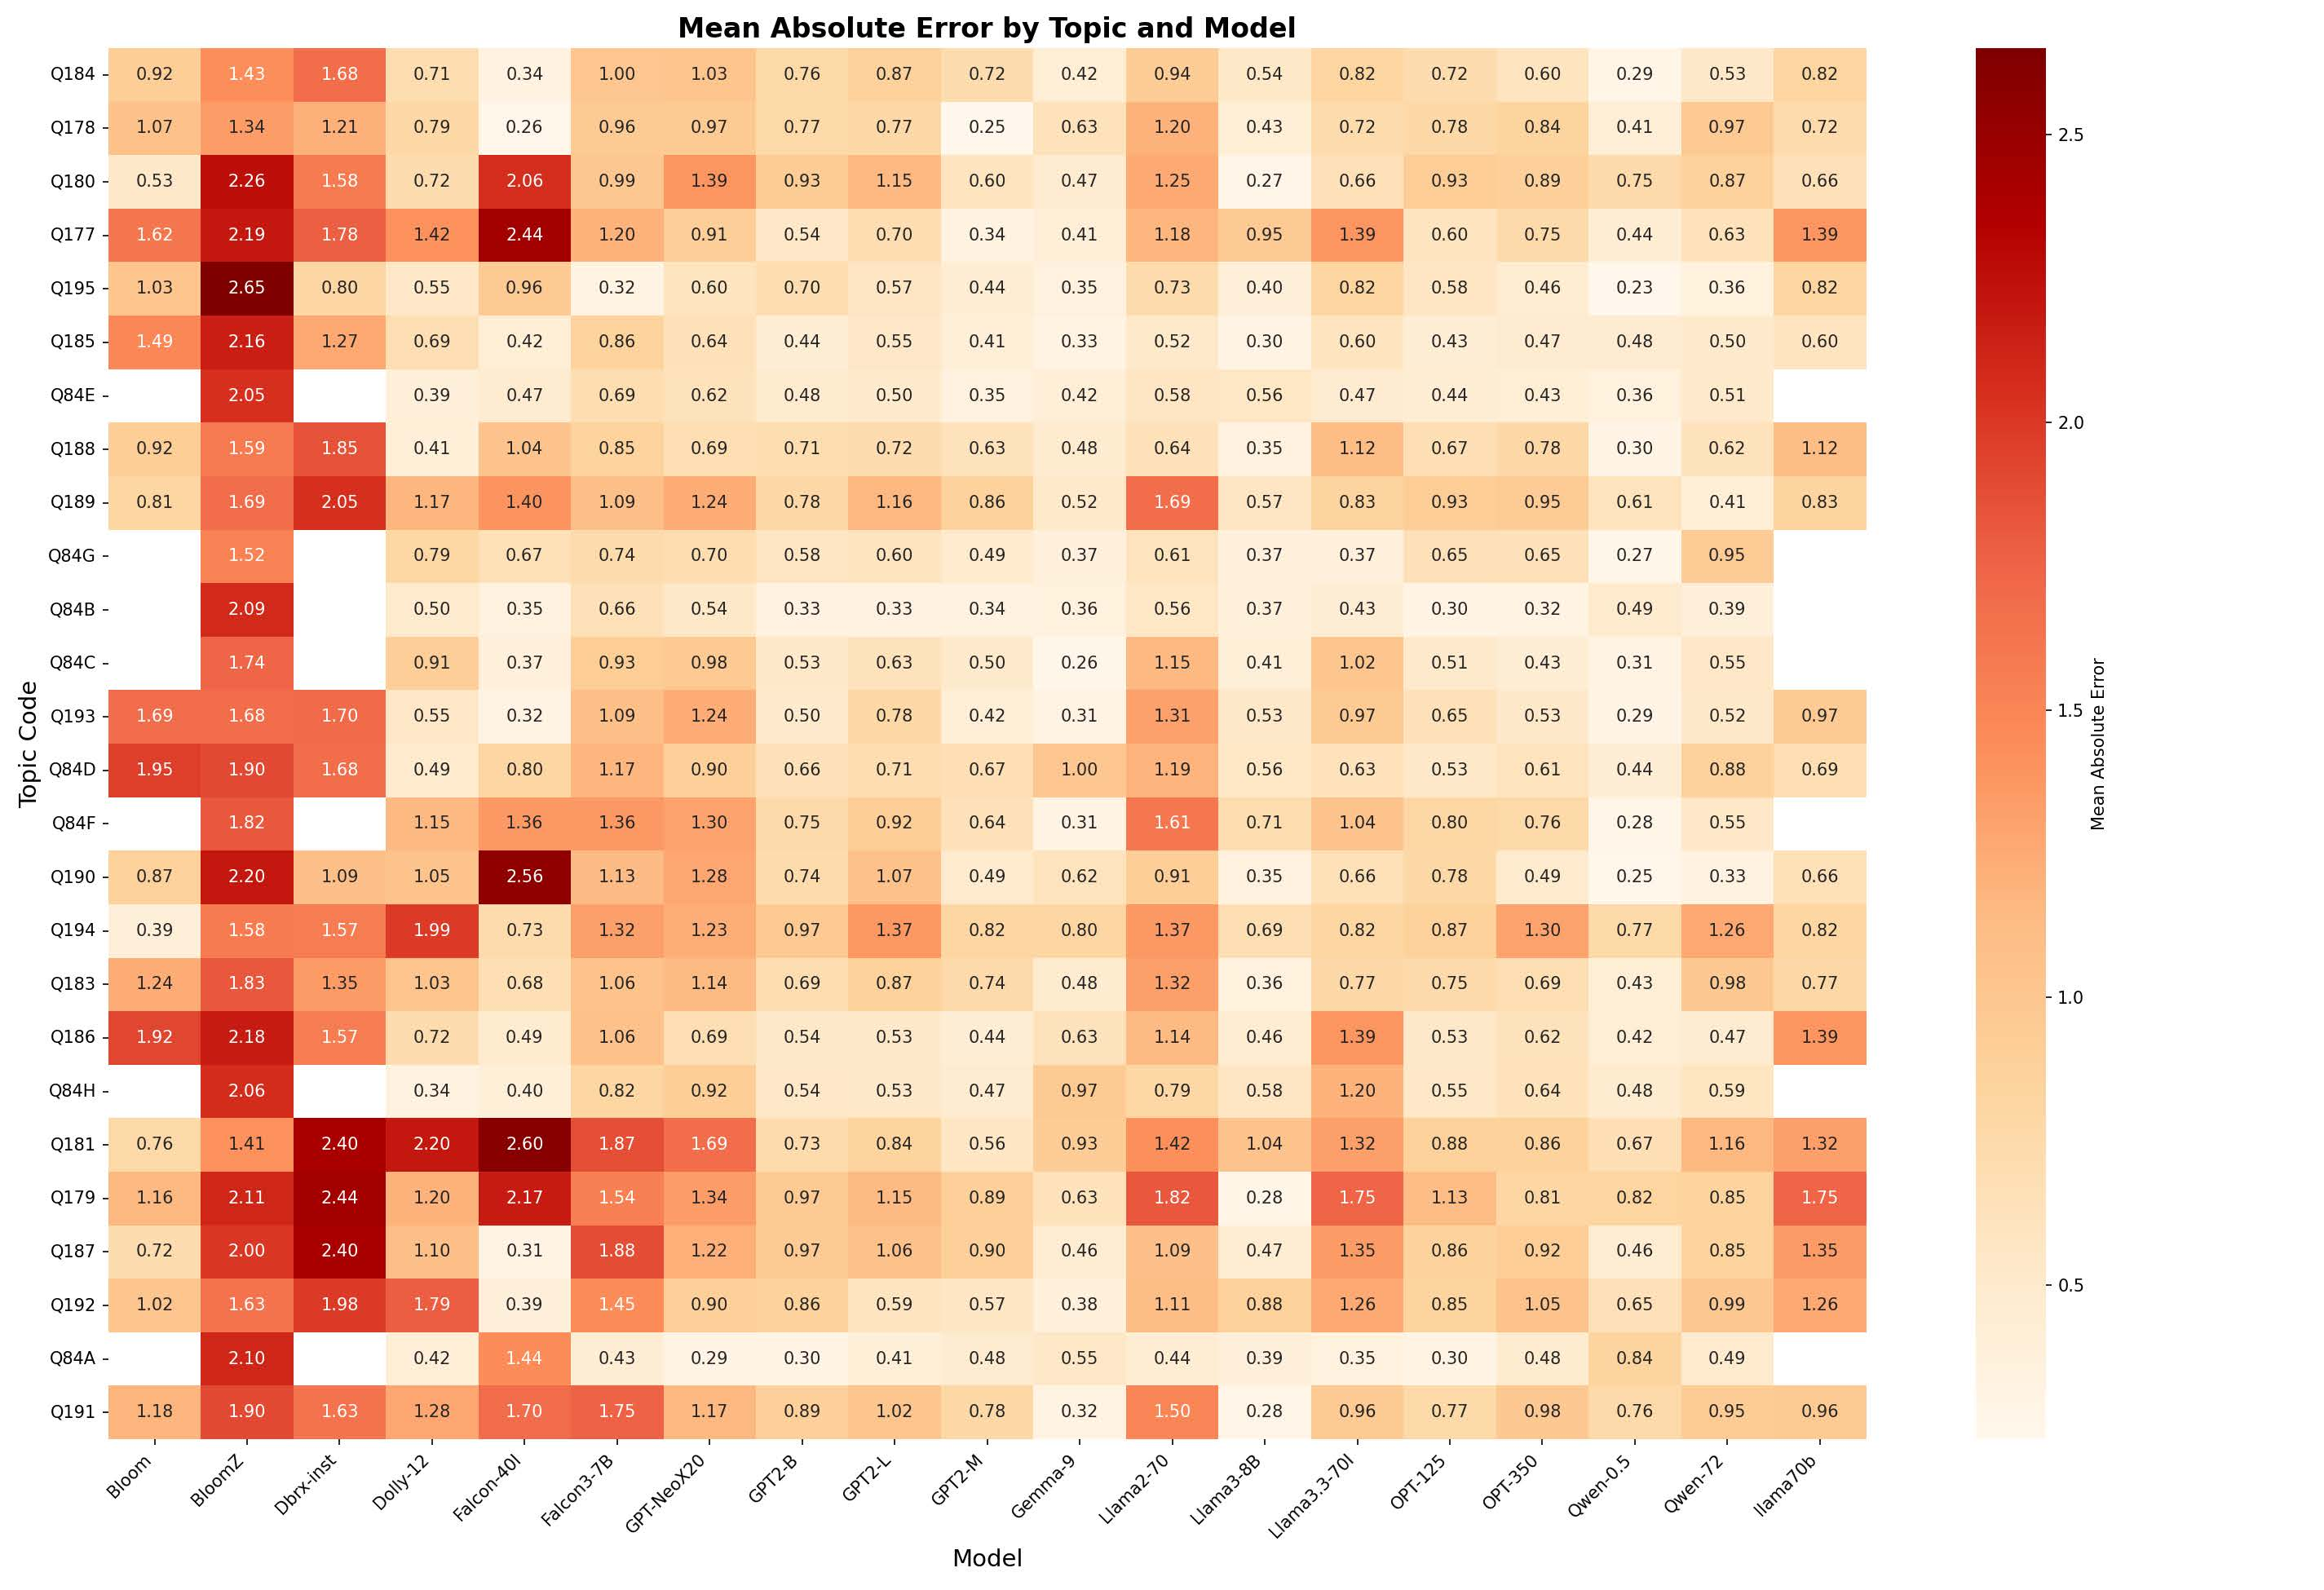
\includegraphics[width=0.85\linewidth]{figures/mean_abs_error_heatmap.pdf}
  \caption{Mean absolute error by topic (rows) and model (columns). Darker cells indicate higher error.}
  \label{fig:heatmap}
\end{figure}


\begin{table}[t]
\centering
\small
\caption{Ten easiest topics (lowest mean absolute error across models).}
\label{tab:EasiestTopics}
\begin{tabularx}{\textwidth}{@{} c Y S[table-format=1.3] S[table-format=1.3] @{}}
\toprule
\# & Topic & {Avg.\ Error} & {Std.\ Dev.} \\
\midrule
1  & Using contraceptives                         & 0.511 & 0.211 \\
2  & Gambling                                     & 0.491 & 0.163 \\
3  & Drinking alcohol                             & 0.482 & 0.112 \\
4  & Parents beating children                     & 0.462 & 0.262 \\
5  & Getting a divorce                            & 0.431 & 0.082 \\
6  & Having casual sex                            & 0.408 & 0.208 \\
7  & Divorce                                      & 0.391 & 0.072 \\
8  & Claiming government benefits not entitled    & 0.386 & 0.199 \\
9  & Euthanasia                                   & 0.384 & 0.079 \\
10 & Death penalty                                & 0.363 & 0.147 \\
\bottomrule
\end{tabularx}
\end{table}

\begin{table}[t]
\centering
\small
\caption{Ten hardest topics (highest mean absolute error across models).}
\label{tab:HardestTopics}
\begin{tabularx}{\textwidth}{@{} c Y S[table-format=1.3] S[table-format=1.3] @{}}
\toprule
\# & Topic & {Avg.\ Error} & {Std.\ Dev.} \\
\midrule
1  & Political violence                           & 0.955 & 0.365 \\
2  & Suicide                                      & 0.923 & 0.249 \\
3  & Stealing property                            & 0.839 & 0.342 \\
4  & Someone accepting a bribe                    & 0.800 & 0.374 \\
5  & For a man to beat his wife                   & 0.782 & 0.288 \\
6  & Cheating on taxes                            & 0.717 & 0.362 \\
7  & Violence against other people                & 0.709 & 0.332 \\
8  & Terrorism (political/ideological)            & 0.692 & 0.281 \\
9  & Homosexuality                                & 0.606 & 0.167 \\
10 & Abortion                                     & 0.599 & 0.310 \\
\bottomrule
\end{tabularx}
\end{table}



%\vspace{-0.8em}
\section{Discussion}
\label{sec:discussion_Conclusion}
%\vspace{-0.8em}
Our findings show considerable variation in how well language models replicate cross-cultural moral judgments, as captured in the WVS and PEW surveys. Larger or instruction tuned models, such as \texttt{Falcon-40I}, \texttt{Gemma-9}, and \texttt{GPT4o}, frequently demonstrate higher correlations with aggregated human survey responses. In contrast, some models, including \texttt{Qwen-0.5} and \texttt{Llama2-70}, yield systematically negative correlations, suggesting that scale alone does not guarantee alignment with moral attitudes if the underlying training data or methodology is insufficiently diverse or biased.

Topic-level analysis reveals that certain issues, such as political violence, terrorism, or wife-beating, consistently produce higher mean errors across different architectures. These discrepancies suggest that moral questions involving violence or extreme social norms may pose particular challenges for current language models, especially when training data do not include nuanced representations of such topics. Even models that perform relatively well on broad measures sometimes fail on region-specific or contentious issues. This trend aligns with evidence that LLMs handle clear-cut moral scenarios well but often display uncertainty or divergence on morally ambiguous dilemmas~\cite{scherrer2023evaluating}. Per-country heatmaps similarly highlight that no single model excels in all areas: while a model may align with opinions in Western nations, it can deviate markedly in communities whose moral or cultural practices are underrepresented in its training corpora.

Despite these limitations, instruction tuned and larger models show promise in better reflecting moral consensus in many cases. This suggests that scaling models and using tailored training that captures diverse viewpoints can improve moral judgment alignment. However, performance still varies, highlighting the need to analyze results in detail (e.g., by topic or country) rather than relying on a single global metric. From an applied perspective, these insights can guide the development of more culturally responsive AI systems, for example, informing content moderation policies or chatbot designs that respect regional norms.


%\vspace{-0.8em}
\section{Conclusion and Limitations}
%\vspace{-0.8em}
In conclusion, our analysis of moral stance alignment across WVS and PEW data underscores both the progress and the continuing gaps in LLMs' performance. Models with substantial parameter counts and instruction tuned frameworks frequently achieve moderate-to-high correlations with surveyed human judgments, suggesting an ability to capture broad moral viewpoints. However, sizable deviations persist on sensitive topics and in particular cultural contexts, indicating that no current model entirely overcomes biases or data deficiencies. Thus, while larger or more specialized training procedures can improve a model's capacity to reflect human moral attitudes, they do not guarantee universal alignment. Future work must address these persistent shortcomings through expanded training corpora, targeted bias mitigation, and refined evaluation protocols that account for cultural and topic-level nuances.

% \vspace{-0.8em}
% \subsection{Limitations}
% \label{sec:limitations}

Although our methodology offers insights into cross-cultural moral alignment in language models, it has several limitations that should be acknowledged. First, the WVS and PEW data capture broad national averages and may not fully reflect within-country heterogeneity, especially in regions with significant cultural or linguistic diversity. Second, our log-probability difference calculation relies on short prompt templates, which might not elicit the full context required for more complex moral issues. Third, the models we evaluated differ in size, instruction tuning, and training data composition, making it challenging to isolate the effect of each factor. Future work could explore alternative elicitation strategies or establish standardized metrics that enable more consistent comparisons across models and prompting approaches.

% A further limitation arises from the necessity of employing distinct evaluation strategies. For local models, we have access to token-level log probabilities, enabling us to compute log-probability differences as a proxy for moral judgment. However, for OpenAI's proprietary chat models, we rely on directly elicited numerical scores because the API does not expose internal log probabilities. This divergence means that the resulting moral scores are derived from different underlying mechanisms, precluding a direct, unified comparison of model outputs in our visualizations. Future work might seek alternative methods to bridge this gap or develop metrics that are comparable across elicitation approaches.

% \begin{credits}
% \subsubsection{\ackname} This research received no external funding. We thank the maintainers of the WVS and PEW data for enabling large-scale cross-cultural analysis. We also thank anonymous reviewers for their valuable comments and feedback and anonymous contributors for their editorial contributions to this paper. We also thank SURF for providing the computational facilities.

% \subsubsection{\discintname}
% The authors declare no conflict of interest.
% \end{credits}
%
% ---- Bibliography ----
%
% BibTeX users should specify bibliography style 'splncs04'.
% References will then be sorted and formatted in the correct style.
%
% \bibliographystyle{splncs04}
% \bibliography{references}

\clearpage

%\appendix
%/here
%\newpage

% ------------------- Appendices (count toward page limit) -------------------
% ------------------- Appendices (count toward page limit) -------------------
\ifincludeappendix
\clearpage
\appendix

\section{Topic Codes for WVS and PEW}
\label{appendix:topic_codes}
\begin{table}[t]
\centering
\small
\caption{Topic codes mapped to WVS and PEW moral questions.}
\label{tab:topic_mapping}
\begin{tabularx}{\textwidth}{@{} c c Y @{}}
\toprule
\textbf{Code} & \textbf{Dataset} & \textbf{Moral Question} \\
\midrule
\multicolumn{3}{c}{\textbf{WVS}}\\
\midrule
Q177 & WVS & Claiming government benefits to which you are not entitled \\
Q178 & WVS & Avoiding a fare on public transport \\
Q179 & WVS & Stealing property \\
Q180 & WVS & Cheating on taxes \\
Q181 & WVS & Someone accepting a bribe in the course of their duties \\
Q182 & WVS & Homosexuality \\
Q183 & WVS & Prostitution \\
Q184 & WVS & Abortion \\
Q185 & WVS & Divorce \\
Q186 & WVS & Sex before marriage \\
Q187 & WVS & Suicide \\
Q188 & WVS & Euthanasia \\
Q189 & WVS & For a man to beat his wife \\
Q190 & WVS & Parents beating children \\
Q191 & WVS & Violence against other people \\
Q192 & WVS & Terrorism as a political, ideological or religious means \\
Q193 & WVS & Having casual sex \\
Q194 & WVS & Political violence \\
Q195 & WVS & Death penalty \\
\midrule
\multicolumn{3}{c}{\textbf{PEW Global Attitudes Survey}}\\
\midrule
Q84A & PEW & Using contraceptives \\
Q84B & PEW & Getting a divorce \\
Q84C & PEW & Having an abortion \\
Q84D & PEW & Homosexuality \\
Q84E & PEW & Drinking alcohol \\
Q84F & PEW & Married people having an affair \\
Q84G & PEW & Gambling \\
Q84H & PEW & Sex between unmarried adults \\
\bottomrule
\end{tabularx}
\end{table}


\fi

% ------------------- References (do not count toward page limit) -----------
\clearpage
\bibliographystyle{splncs04}
\bibliography{references}


% Warn on missing citations during draft
\makeatletter
\def\@citex[#1]#2{\leavevmode
  \let\@citea\@empty
  \@cite{\@for\@citeb:=#2\do
    {\@citea\def\@citea{,}\@ifundefined{b@\@citeb}{\textbf{[MISSING:\@citeb]}}{\hbox{\csname b@\@citeb\endcsname}}}{#1}}}
\makeatother




\end{document}